\documentclass{standalone}
\usepackage{tikz}

\usetikzlibrary{fit}

\def\sector#1#2{
      \node (innen) at #1 [draw, minimum width=2cm, minimum height=1cm] {}; 
      \node[xshift=0.75cm, yshift=-0.25cm] at (innen) {#2};
}

\begin{document}
  \nopagecolor
  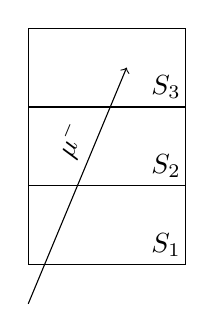
\begin{tikzpicture}
      \sector{(0,0)}{$S_1$}
      \sector{(0,1)}{$S_2$}
      \sector{(0,2)}{$S_3$}

      \draw [->] (-1,-1) -- node [above, sloped, xshift=0.5cm] {$\mu^-$} (0.25,2);
  \end{tikzpicture}
\end{document}
